\documentclass[10pt,final,journal]{IEEEtran}
\usepackage[numbers]{natbib}
\usepackage{graphicx}
\usepackage{lipsum}

\graphicspath{{./img/}}
\title{Room localisation in the Museum of Fine Arts in Ghent using painting recognition}
\author{Bert De Saffel, Timothy Thiecke}
\begin{document}
	\maketitle
	\begin{abstract}
		This paper describes our method to localise a painting on a ground plan based on The Musem of Fine Arts in Ghent. 
	\end{abstract}


	\section{Introduction}
	The Museum of Fine Arts in Ghent houses a large collection of mostly Flemish art such as paintings and sculptures. The museum allows its customers to take photographs or videos of most art pieces for own usage. 
	
	Based on a frame from a ca which contains a painting, 
	
	Figure \ref{fig:groundplan_msk} shows the ground plan that is used to mark the correct room
	
	\begin{figure}
		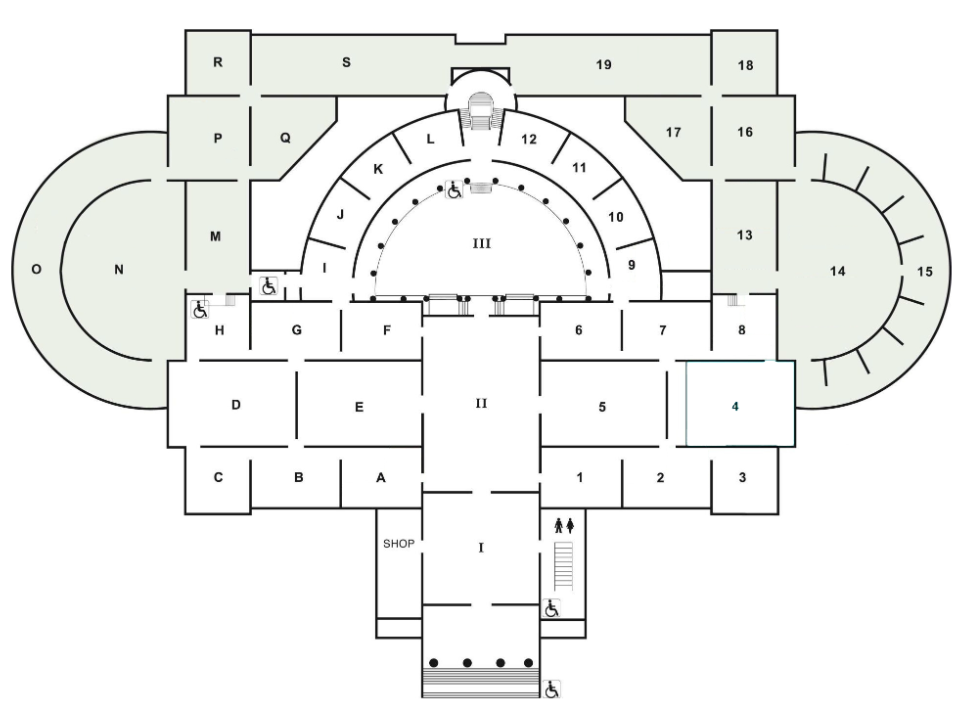
\includegraphics[width=\linewidth]{groundplan_msk}
		\caption{A ground plan of The Museum of Fine Arts, Ghent. }
		\label{fig:groundplan_msk}
	\end{figure}

	
	
	\section{Painting Detection}
	
	\lipsum[6]
	
	\subsection{Painting Segmentation}
	\lipsum[7-11]
	\subsection{Feature detection}
	\lipsum[12-15]
	\section{Results}
	\lipsum[16-18]
	\section{Conclusion}
	\lipsum[19]

	\bibliographystyle{IEEEtran}
	\bibliography{IEEEabrv,library}
\end{document}